% How the selected frames are combined (Section 4.5, "Combining the selected frames", and the LSTM readouts).
% Bar lengths are drawn to scale for k = 3 (1,518 values per frame), except the 3 similarity values, drawn wider to be visible.
\documentclass[12pt,border=10pt]{standalone}
% Shared style for the slide figures: sans-serif text (Helvetica, close to the Arial of the charts),
% the same colors as charts.py, and the manuscript's table tools.
\usepackage[T1]{fontenc}
\usepackage[scaled]{helvet}
\renewcommand{\familydefault}{\sfdefault}
\usepackage{amsmath,amssymb}
\usepackage{sansmath}
\usepackage{xcolor}
\usepackage{booktabs,array}
\newcolumntype{L}[1]{>{\raggedright\arraybackslash}p{#1}}
\usepackage{tikz}
\usetikzlibrary{arrows.meta,positioning,calc}

\definecolor{ink}{HTML}{0B0B0B}
\definecolor{inktwo}{HTML}{52514E}
\definecolor{muted}{HTML}{898781}
\definecolor{gridc}{HTML}{E1E0D9}
\definecolor{basec}{HTML}{C3C2B7}
% one color per selection rule, in the fixed categorical order of the charts
\definecolor{cp}{HTML}{2A78D6}     % k-Changepoint (content)
\definecolor{sme}{HTML}{EB6834}    % SME (position)
\definecolor{posc}{HTML}{1BAF7A}    % positional (position)
\definecolor{rnd}{HTML}{EDA100}    % random (chance)
\definecolor{bocpd}{HTML}{E87BA4}  % k-BOCPD (content), categorical slot 5
\definecolor{temporal}{HTML}{6250D6}  % temporal information added to the mean (frame combinations figure)

\newcommand{\chip}[1]{\tikz[baseline=0.1ex]\fill[#1, rounded corners=1pt] (0,0) rectangle (0.32cm,0.32cm);}
\AtBeginDocument{\sansmath\color{ink}}
\hyphenpenalty=10000 \exhyphenpenalty=10000   % no hyphenated words on slides

\newcommand{\fvec}[4]{% #1 x start, #2 y centre, #3 length, #4 fill
   \draw[white, line width=1pt, fill=#4] (#1, #2-0.17) rectangle (#1+#3, #2+0.17);}
\begin{document}
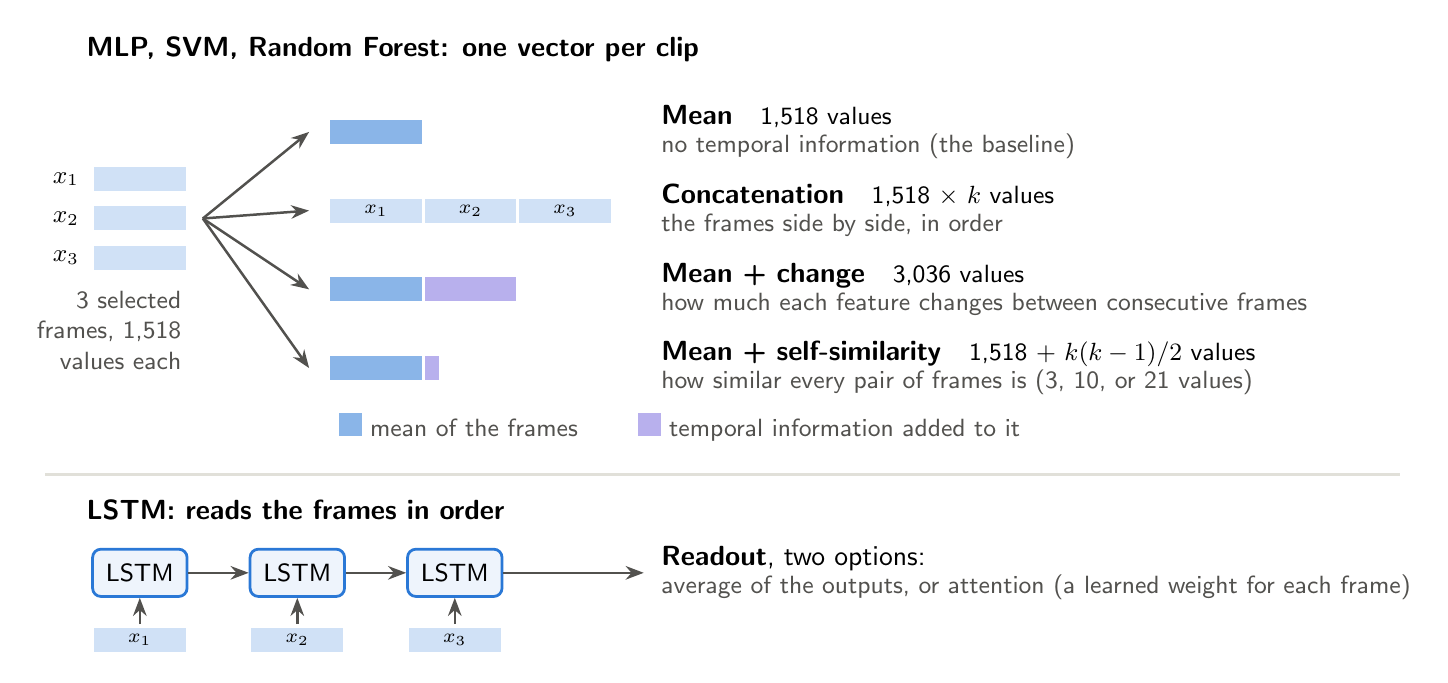
\begin{tikzpicture}[arr/.style={-{Stealth[length=2.3mm]}, line width=0.9pt, color=inktwo}]
   % ---------- MLP, SVM, Random Forest
   \node[anchor=west, font=\normalsize\bfseries] at (-0.2, 2.25) {MLP, SVM, Random Forest: one vector per clip};
   \node[anchor=north east, font=\small, text=inktwo, align=right] at (1.25, -0.7) {3 selected\\frames, 1,518\\values each};
   \foreach \y/\n in {0.6/1, 0.1/2, -0.4/3} {
      \fvec{0}{\y}{1.2}{cp!22}
      \node[anchor=east, font=\small] at (-0.05, \y) {$x_{\n}$};
   }
   \foreach \y in {1.2, 0.2, -0.8, -1.8} \draw[arr] (1.4, 0.1) -- (2.75, \y);
   % mean
   \fvec{3.0}{1.2}{1.2}{cp!55}
   \node[anchor=west, align=left] at (7.1, 1.2) {\textbf{Mean}\quad\small 1,518 values\\[-2pt]\small\textcolor{inktwo}{no temporal information (the baseline)}};
   % concatenation
   \fvec{3.0}{0.2}{1.2}{cp!22} \fvec{4.2}{0.2}{1.2}{cp!22} \fvec{5.4}{0.2}{1.2}{cp!22}
   \node[font=\scriptsize] at (3.6, 0.2) {$x_1$}; \node[font=\scriptsize] at (4.8, 0.2) {$x_2$}; \node[font=\scriptsize] at (6.0, 0.2) {$x_3$};
   \node[anchor=west, align=left] at (7.1, 0.2) {\textbf{Concatenation}\quad\small 1,518 $\times$ $k$ values\\[-2pt]\small\textcolor{inktwo}{the frames side by side, in order}};
   % mean and change
   \fvec{3.0}{-0.8}{1.2}{cp!55} \fvec{4.2}{-0.8}{1.2}{temporal!45}
   \node[anchor=west, align=left] at (7.1, -0.8) {\textbf{Mean + change}\quad\small 3,036 values\\[-2pt]\small\textcolor{inktwo}{how much each feature changes between consecutive frames}};
   % mean and self-similarity
   \fvec{3.0}{-1.8}{1.2}{cp!55} \fvec{4.2}{-1.8}{0.22}{temporal!45}
   \node[anchor=west, align=left] at (7.1, -1.8) {\textbf{Mean + self-similarity}\quad\small 1,518 + $k(k-1)/2$ values\\[-2pt]\small\textcolor{inktwo}{how similar every pair of frames is (3, 10, or 21 values)}};
   % key
   \node[anchor=west, font=\small, text=inktwo] at (3.0, -2.55)
      {\textcolor{cp!55}{\rule{0.9em}{0.9em}}\ mean of the frames \qquad \textcolor{temporal!45}{\rule{0.9em}{0.9em}}\ temporal information added to it};

   % ---------- LSTM
   \draw[gridc, line width=1pt] (-0.6, -3.15) -- (16.6, -3.15);
   \node[anchor=west, font=\normalsize\bfseries] at (-0.2, -3.6) {LSTM: reads the frames in order};
   \foreach \x/\n in {0.0/1, 2.0/2, 4.0/3} {
      \fvec{\x}{-5.25}{1.2}{cp!22}
      \node[font=\scriptsize] at (\x+0.6, -5.25) {$x_{\n}$};
      \node[draw=cp, fill=cp!8, line width=1pt, rounded corners=3pt, minimum width=1.2cm, minimum height=0.6cm, font=\small] (c\n) at (\x+0.6, -4.4) {LSTM};
      \draw[arr] (\x+0.6, -5.05) -- (c\n.south);
   }
   \draw[arr] (c1) -- (c2);
   \draw[arr] (c2) -- (c3);
   \draw[arr] (c3.east) -- (7.0, -4.4);
   \node[anchor=west, align=left] at (7.1, -4.4) {\textbf{Readout}, two options:\\[-2pt]\small\textcolor{inktwo}{average of the outputs, or attention (a learned weight for each frame)}};
\end{tikzpicture}
\end{document}
